\documentclass{beamer}
\usetheme{Boadilla}
\usepackage{tikz}
\usepackage{graphicx}



\title{Weekly Presentation}
\subtitle{Week 40}
\author{}
\institute{Luleå University of Technology}
\date{\today}



\begin{document}
\begin{frame}
    \titlepage
\end{frame}


%%%%%%%%%%%%%%%% new page %%%%%%%%%%%%%%%%%%%%%%


\begin{frame}
    \subsection{Group members}
    \frametitle{Group members }
    \begin{itemize}
        \item Y-students
        \begin{itemize}
            \item Martin Blaszczyk - Project leader and object detection
            \item Edward Cedergård -Arm and gripping tool
            \item Niklad Dahlqvist -  Arm and gripping tool
            \item Måns Norell - Movable base
        \end{itemize}
        \item D-students
        \begin{itemize}
            \item Edward Källstedt - Object detection
            \item Albin Martinsson - Arrowhead and Git
        \end{itemize}  
    \end{itemize}
\end{frame}


%%%%%%%%%%%%%%%% new page %%%%%%%%%%%%%%%%%%%%%%


\begin{frame}{Overview}
What we have done and what we are working on:
    \begin{itemize}
        \item Duplex to simplex
        \item Serial communication
        \item Dynamixel data packages
        \item Arm construction
    \end{itemize}
\end{frame}


%%%%%%%%%%%%%%%% new page %%%%%%%%%%%%%%%%%%%%%%



%%%%%%%%%%%%%%%% new page %%%%%%%%%%%%%%%%%%%%%%

\begin{frame}{Full-duplex to half-duplex }

    \begin{figure}
        \centering
        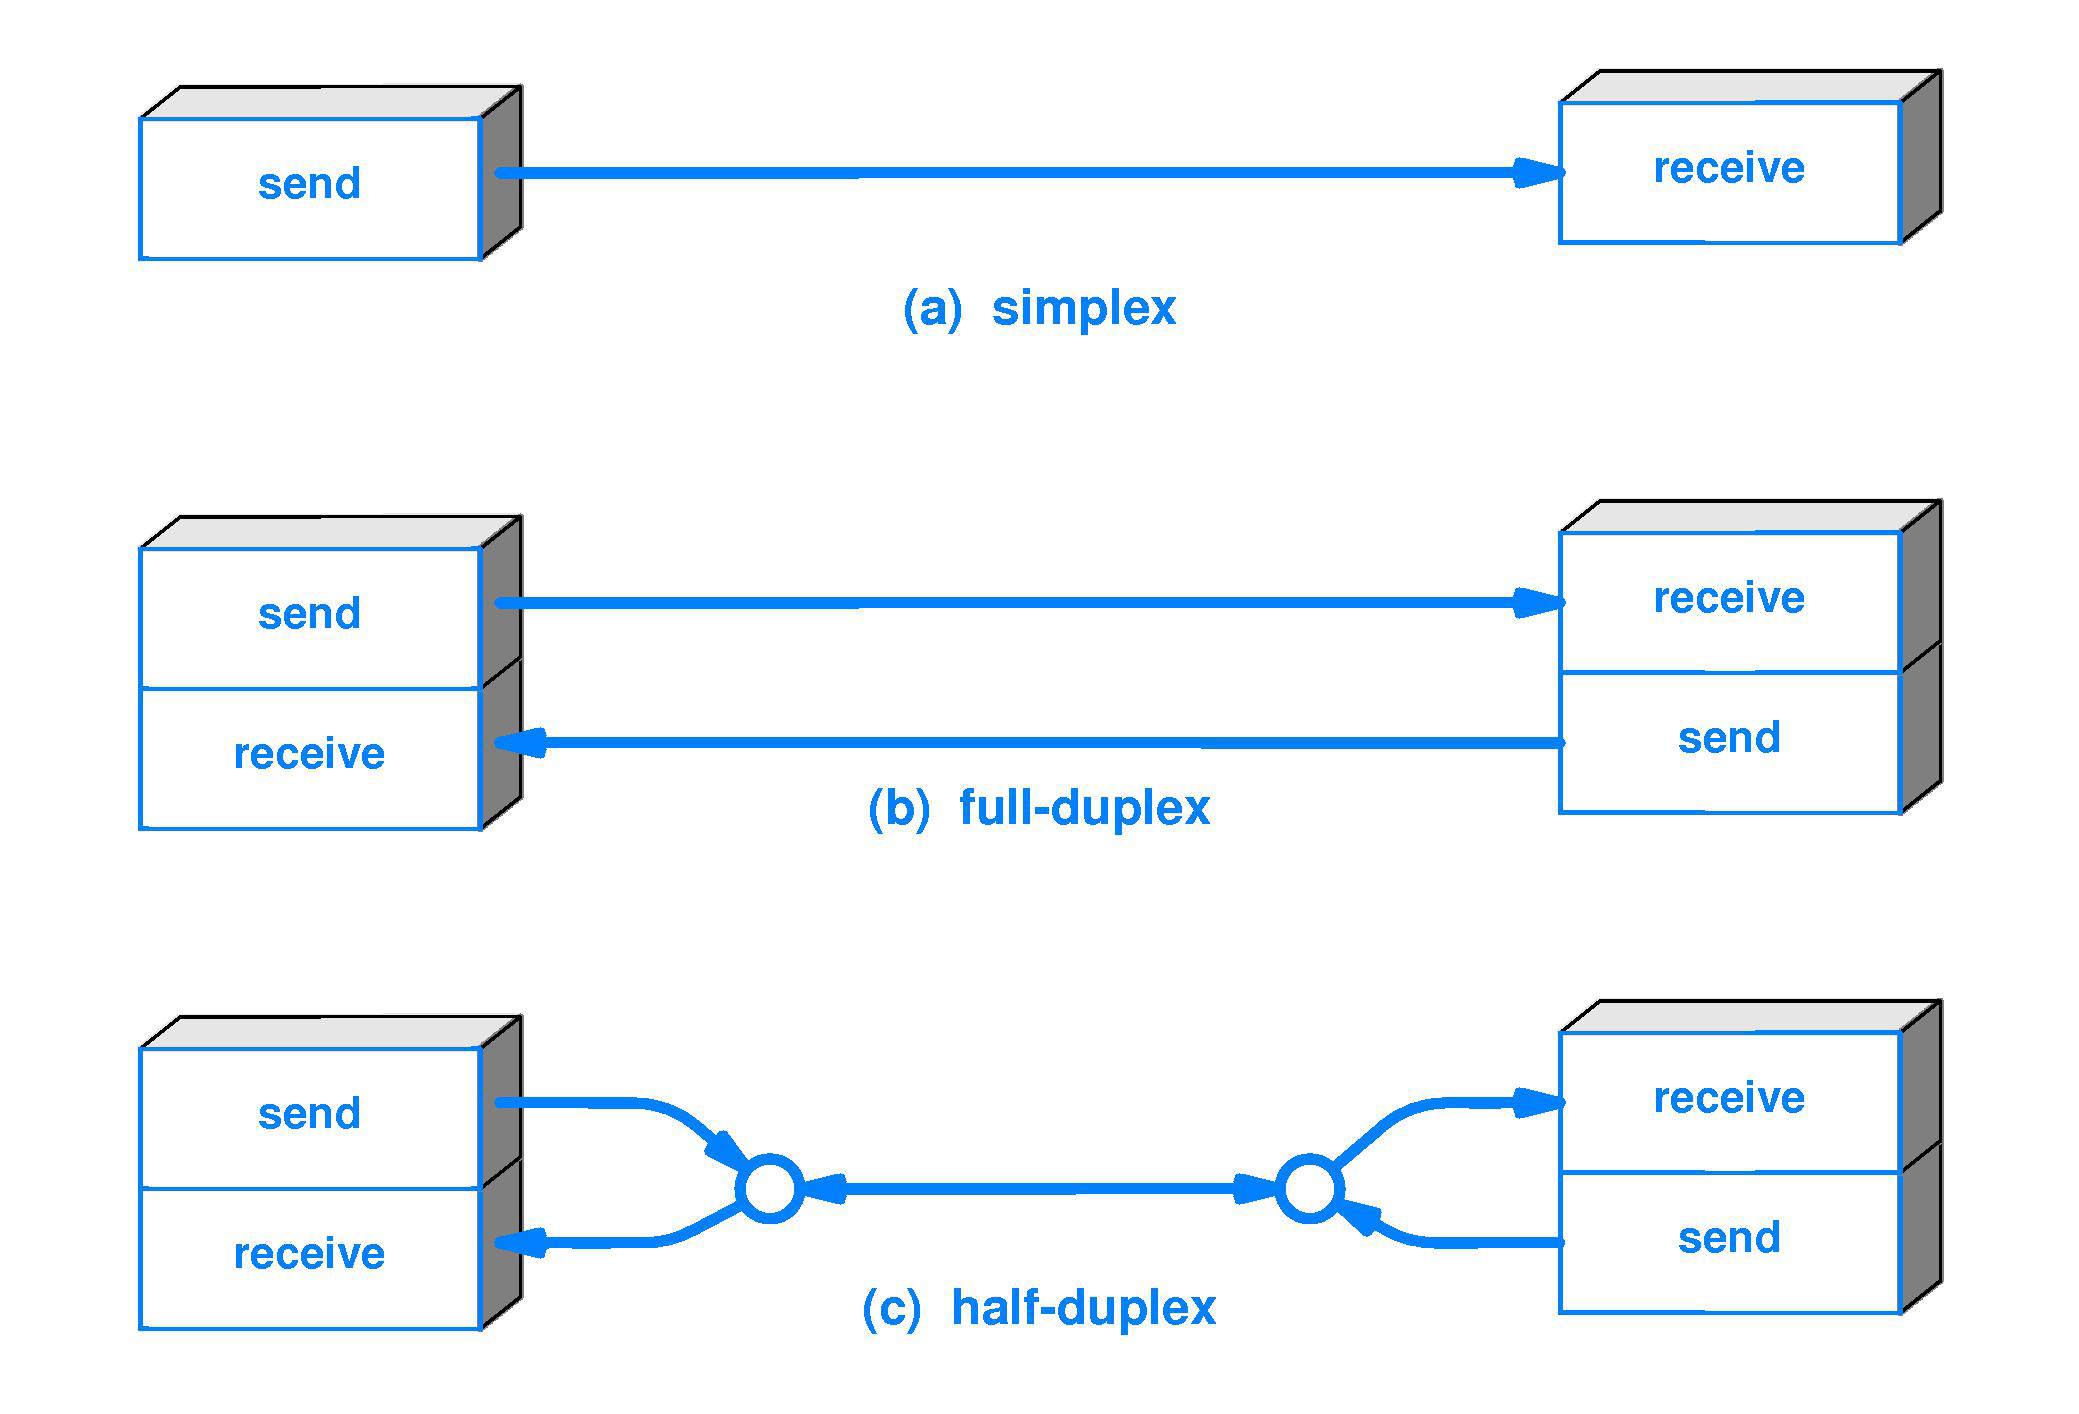
\includegraphics[width = \textwidth]{img/BBE_Simplex vs Duplex_Transmissions.jpg}
        
    \end{figure}
    
\end{frame}


%%%%%%%%%%%%%%%% new page %%%%%%%%%%%%%%%%%%%%%%

\begin{frame}{Dynamixel communication}

    \begin{figure}
        \centering
        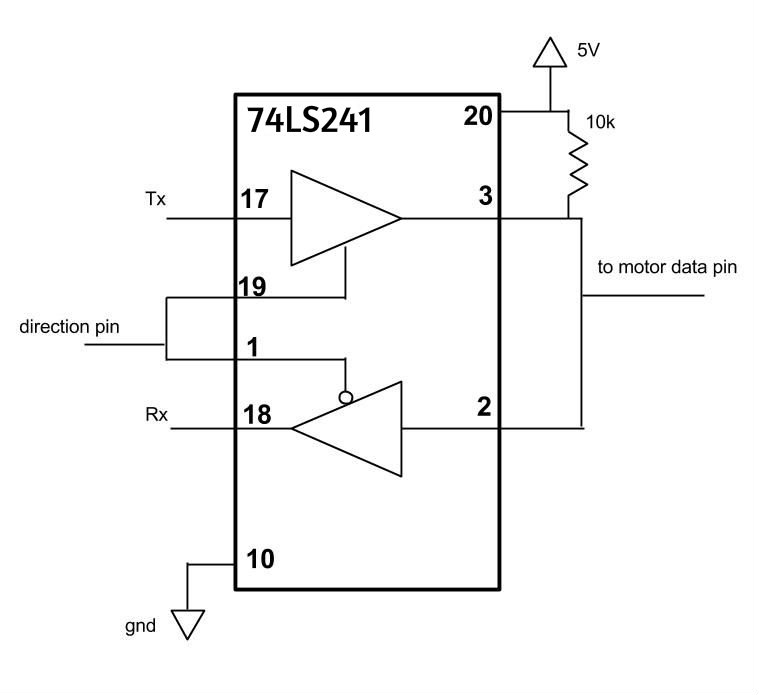
\includegraphics[width =9.5cm]{img/uart_half-duplex_74LS241.jpg}
        
    \end{figure}
    
\end{frame}


%%%%%%%%%%%%%%%% new page %%%%%%%%%%%%%%%%%%%%%%

\begin{frame}{Curcuit}

    \begin{figure}
        \centering
        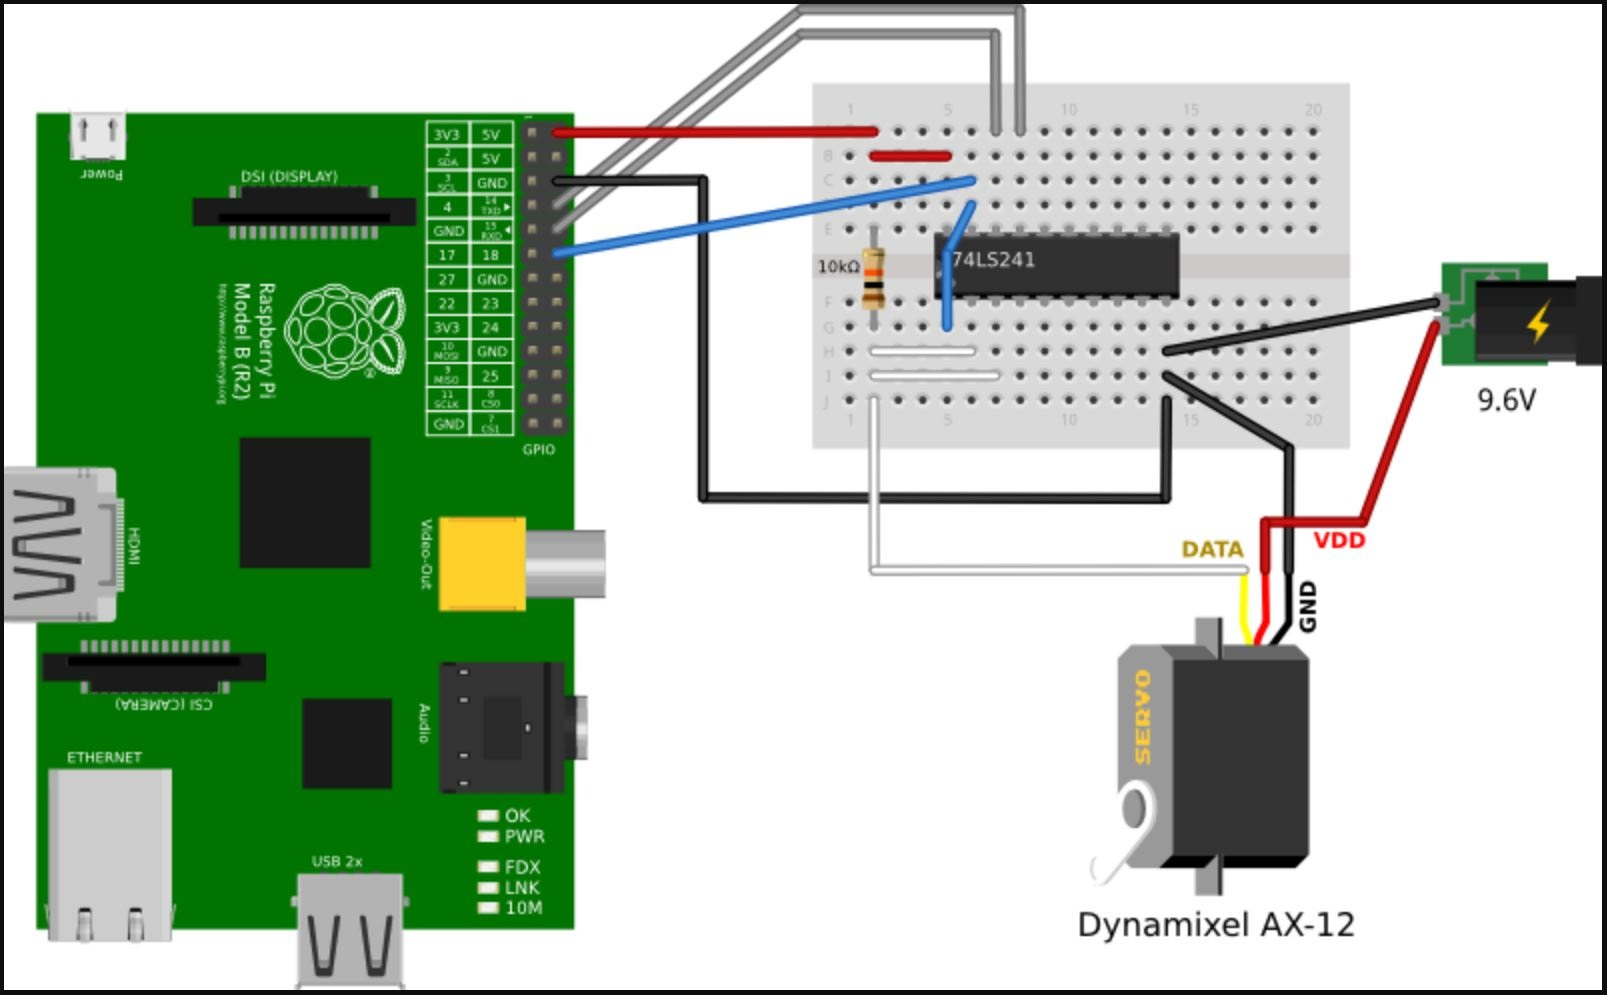
\includegraphics[width = \textwidth]{img/curcuit.jpg}
        
    \end{figure}
    
\end{frame}


%%%%%%%%%%%%%%%% new page %%%%%%%%%%%%%%%%%%%%%%

\begin{frame}{Serial communication}

    \begin{columns}
        \begin{column}[]{0.5\textwidth}
            \begin{itemize}
                \item Logic analyzer
            \end{itemize}
        \end{column}
        
        
        \begin{column}[]{0.5\textwidth}
        \end{column}
    \end{columns}
    
\end{frame}

%%%%%%%%%%%%%%%% new page %%%%%%%%%%%%%%%%%%%%%%


\begin{frame}{Dynamixel data packages}

    \begin{columns}
        \begin{column}[]{0.5\textwidth}
            \begin{itemize}
                \item Data packets structure
                \item Timing of response
                \item Example package
            \end{itemize}
        \end{column}
        
        
        \begin{column}[]{0.5\textwidth}
        \end{column}
    \end{columns}
    
\end{frame}

%%%%%%%%%%%%%%%% new page %%%%%%%%%%%%%%%%%%%%%%


\begin{frame}{Dynamixel data packages}
    Instruction package - send to the motor
    \begin{table}
        \begin{tabular}{| c | c | c | c | c | c | c | c |}
            \hline
            Header & ID & Length & Instruction & Param 1 & ... & Param n & Checksum\\
            \hline
            0xFFFF & ID & Length & Instruction & param 1 & ... & Param n & Checksum\\
            \hline
        \end{tabular}
    \end{table}
    
    Status return package - recieve from the motor

    \begin{table}
        \begin{tabular}{| c | c | c | c | c | c | c | c |}
            \hline
            Header & ID & Length & Error & Param 1 & ... & Param n & Checksum\\
            \hline
            0xFFFF & ID & Length & Error & Param 1 & ... & Param n & Checksum\\
            \hline
        \end{tabular}
    \end{table}
    
\end{frame}


%%%%%%%%%%%%%%%% new page %%%%%%%%%%%%%%%%%%%%%%


\begin{frame}{Instruction package}
    
        \begin{table}
            \begin{flushleft}
                \begin{tabular}{| c |}
                    \hline
                    Header\\
                    \hline
                    0xFFFF\\
                    \hline
                \end{tabular}
            \end{flushleft}
        \end{table}

\end{frame}


%%%%%%%%%%%%%%%% new page %%%%%%%%%%%%%%%%%%%%%%


\begin{frame}{Instruction package}
 
    \begin{table}
        \begin{flushleft}
            \begin{tabular}{| c | c | c |}
                \hline
                Header & ID & Length\\
                \hline
                0xFFFF & ID & Length \\
                \hline
            \end{tabular}
        \end{flushleft}
    \end{table}
    
\end{frame}



%%%%%%%%%%%%%%%% new page %%%%%%%%%%%%%%%%%%%%%%


\begin{frame}{Instruction package}
 
    \begin{table}
        \begin{flushleft}
            \begin{tabular}{| c | c | c | c | c | c | c |}
                \hline
                Header & ID & Length & Instruction & Param 1 & ... & Param n\\
                \hline
                0xFFFF & ID & Length & Instruction & param 1 & ... & Param n\\
                \hline
            \end{tabular}
        \end{flushleft}
    \end{table}
    
\end{frame}


%%%%%%%%%%%%%%%% new page %%%%%%%%%%%%%%%%%%%%%%


\begin{frame}{Instruction package}

    \begin{table}
        \begin{flushleft}
            \begin{tabular}{| c | c | c | c | c | c | c | c |}
                \hline
                Header & ID & Length & Instruction & Param 1 & ... & Param n & Checksum\\
                \hline
                0xFFFF & ID & Length & Instruction & param 1 & ... & Param n & Checksum\\
                \hline
            \end{tabular}
        \end{flushleft}
    \end{table}
    
\end{frame}

%%%%%%%%%%%%%%%% new page %%%%%%%%%%%%%%%%%%%%%%


\begin{frame}{Status return package}

    \begin{table}
        \begin{flushleft}
            \begin{tabular}{| c | c | c | c | c | c | c | c |}
                \hline
                Header & ID & Length & Error & Param 1 & ... & Param n & Checksum\\
                \hline
                0xFFFF & ID & Length & Error & Param 1 & ... & Param n & Checksum\\
                \hline
            \end{tabular}
        \end{flushleft}
    \end{table}
    
\end{frame}

%%%%%%%%%%%%%%%% new page %%%%%%%%%%%%%%%%%%%%%%


\begin{frame}{Timing of return package}

    \begin{itemize}
        \item Return delay can be set for each motor
        \item Values between 0 - 254 \(\)s
    \end{itemize}
    
\end{frame}

%%%%%%%%%%%%%%%% new page %%%%%%%%%%%%%%%%%%%%%%

\begin{frame}{Arm construction}

    \begin{columns}
        \begin{column}[]{0.5\textwidth}
            \begin{itemize}
                \item Use the official plastic pieces
            \end{itemize}
        \end{column}
        
        
        \begin{column}[]{0.5\textwidth}
        \end{column}
    \end{columns}
    
\end{frame}


%%%%%%%%%%%%%%%% new page %%%%%%%%%%%%%%%%%%%%%%



%%%%%%%%%%%%%%%% new page %%%%%%%%%%%%%%%%%%%%%%





%%%%%%%%%%%%%%%% new page %%%%%%%%%%%%%%%%%%%%%%















%%%%%%%%%%%%%%%% new page %%%%%%%%%%%%%%%%%%%%%%


%%%%%%%%%%%%%%%% new page %%%%%%%%%%%%%%%%%%%%%%




%%%%%%%%%%%%%%%%%%%%%%%%%%%%%%%%%%%%%%%%%%%%%%%%%%%%%%%%%%%%%%%%
%%%%%%%%%%%%%%%%%%%%%%%% Time Plan %%%%%%%%%%%%%%%%%%%%%%%%%%%%%
%%%%%%%%%%%%%%%%%%%%%%%%%%%%%%%%%%%%%%%%%%%%%%%%%%%%%%%%%%%%%%%%
\begin{frame}
    \subsection{Time plan}
    \frametitle{Overall timetable}
    \begin{table}
        \begin{tabular}{| l | c | c | c | c }
            
            Sep & Oct & Nov & Dec \\
            \hline \hline
            Concept generation & Evaluation & Evaluation &  \\ 
            \hline
            Theory & Prototyping & Evaluation & Finishing up \\
            \hline
            Simulation & Evaluation & Evaluation & \\
            \hline
            Prototyping & Final Design & Evaluation &  \\
            \hline
 
        \end{tabular}
    \end{table}    
\end{frame}


\begin{frame}
    \frametitle{Time plan for September}
    \begin{table}
        \begin{tabular}{l | c | c | c | c }
        Subproject & Week 1 & Week 2 & Week 3 & Week 4 \\
        \hline \hline
            Arrowhead & Reading& Setup & API & Prototyping\\
            Movable base & Reading& Modeling & Simulation & Implementation\\
            Arm and grip  & Reading & Kinematics & Simulation& Prototyping\\
            Object detection & Reading & Testing & Prototyping & Evaluation\\
        \end{tabular}
    \end{table}
\end{frame}


\begin{frame}
    \begin{center}
        \Huge Questions?
    \end{center}
\end{frame}



\end{document}